Antes de analizar los resultados, es importante destacar la metodología utilizada para la medición de memoria. 
En este trabajo, se consideró únicamente el peak de memoria dinámica (heap) utilizado por cada algoritmo. 
No se considero el stack, ya que este es memoria propia de trabajar con arreglos y no de los algoritmos,
Por esta razón, se decidió excluirlo del análisis.
En el caso de sort, el algoritmo no debería requerir memoria dinámica adicional. 
Sin embargo, en las mediciones realizadas se observó consistentemente un uso de memoria heap equivalente a 4n bytes, es decir, 
exactamente el tamaño de un arreglo de n enteros. Además, al modificar la función para que no retornara el vector y fuera de tipo void, 
dicha memoria adicional desapareció. Esto indica que el consumo registrado no proviene del algoritmo en sí, 
sino de la copia asociada al valor de retorno de la función utilizada en la implementación experimental. 
Por esta razón, dicha memoria fue descontada del análisis, sin modificar la implementación original entregada en el enunciado de la tarea.
\\
A continuación, se presenta el análisis de los algoritmos de ordenamiento de arreglos. 
En particular, se examinan las gráficas obtenidas a partir de los experimentos, con el objetivo de analizar 
el comportamiento temporal y de memoria de cada algoritmo de manera individual.
\begin{figure}[H]
    \centering
    \resizebox{\textwidth}{!}{
        \begin{minipage}{\textwidth}
            \centering

            \begin{subfigure}{0.48\textwidth}
                \centering
                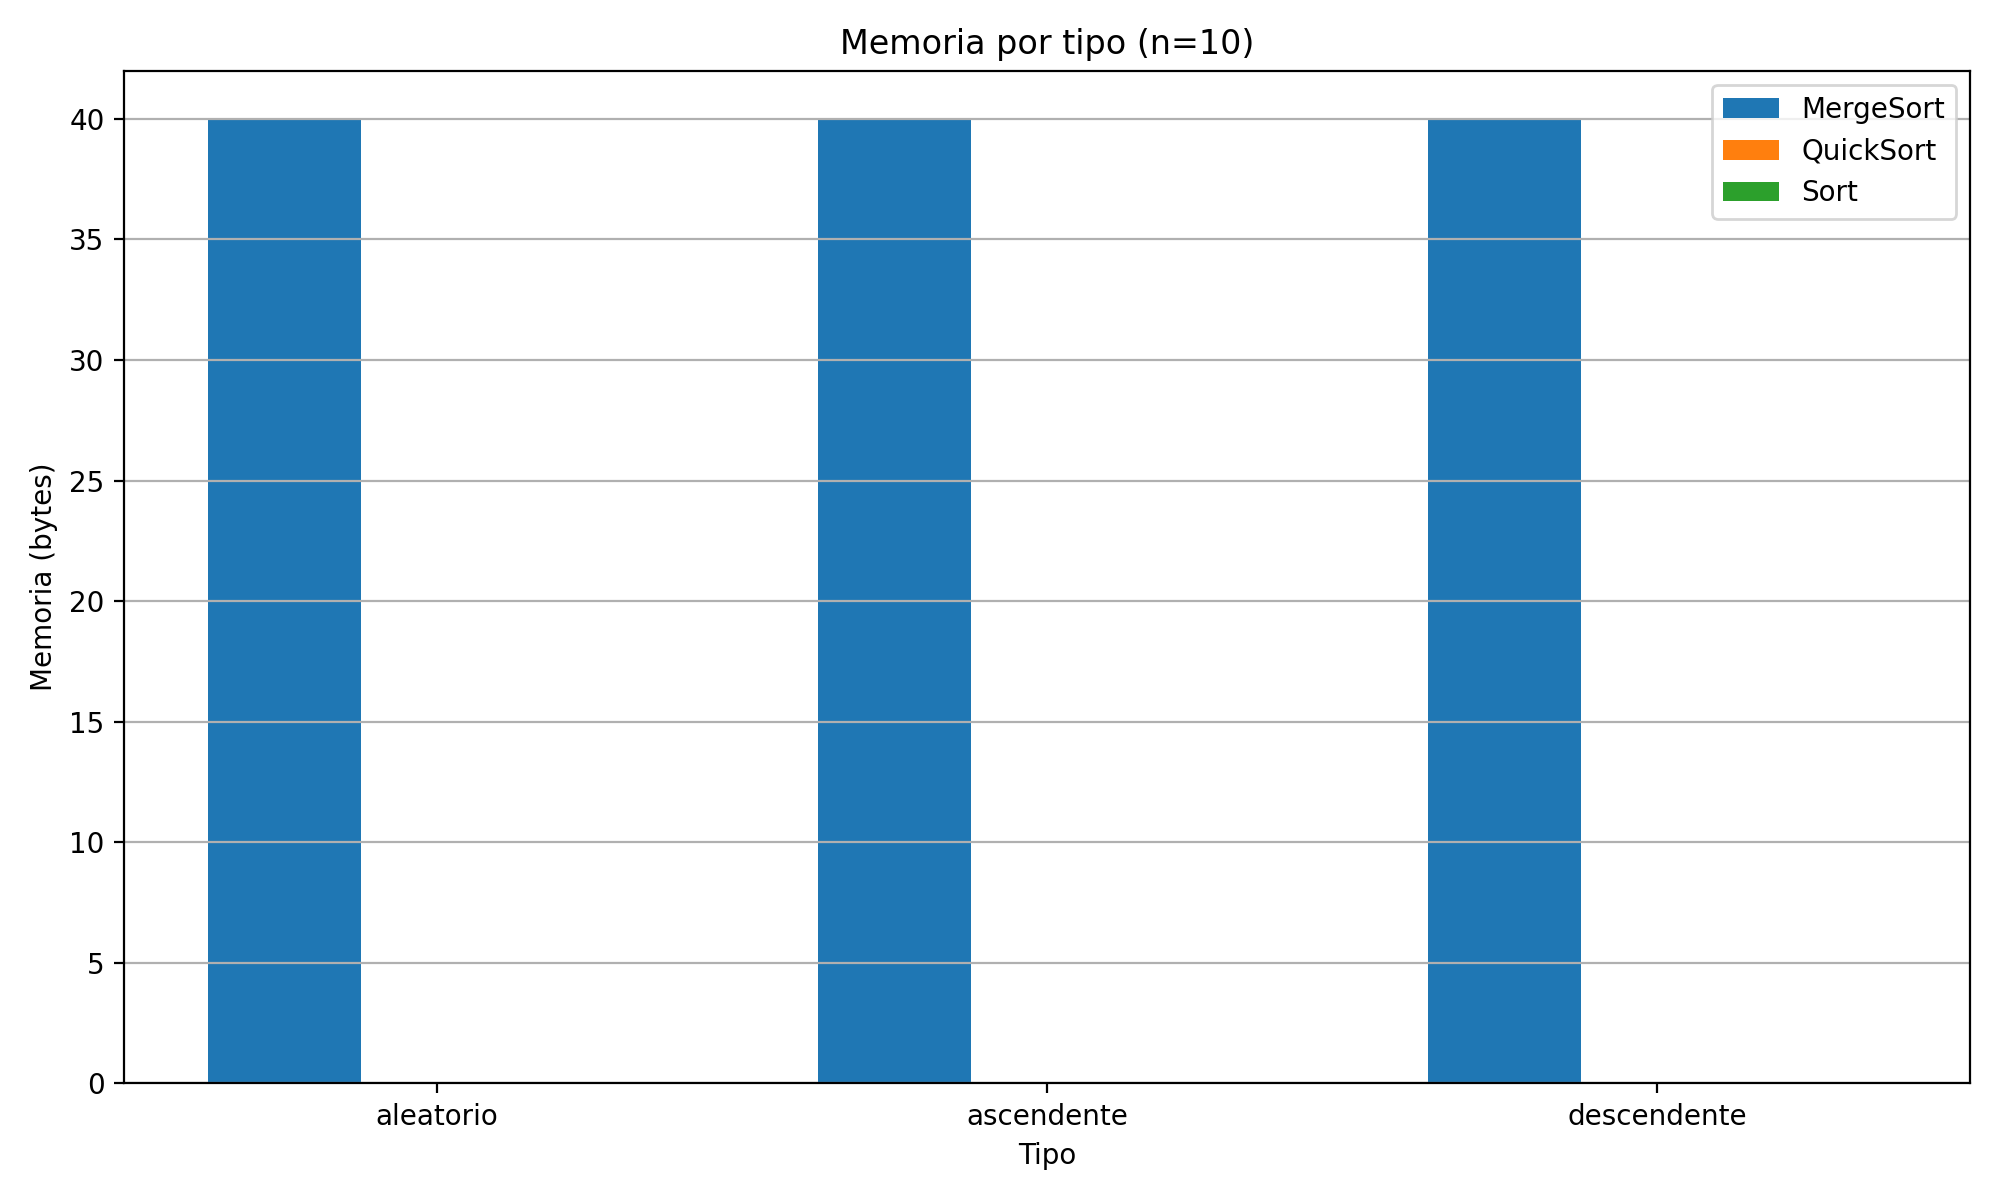
\includegraphics[width=\linewidth]{../code/sorting/data/plots/memory_n10.png}
                \caption{Memoria}
                \label{fig:img1}
            \end{subfigure}
            \hfill
            \begin{subfigure}{0.48\textwidth}
                \centering
                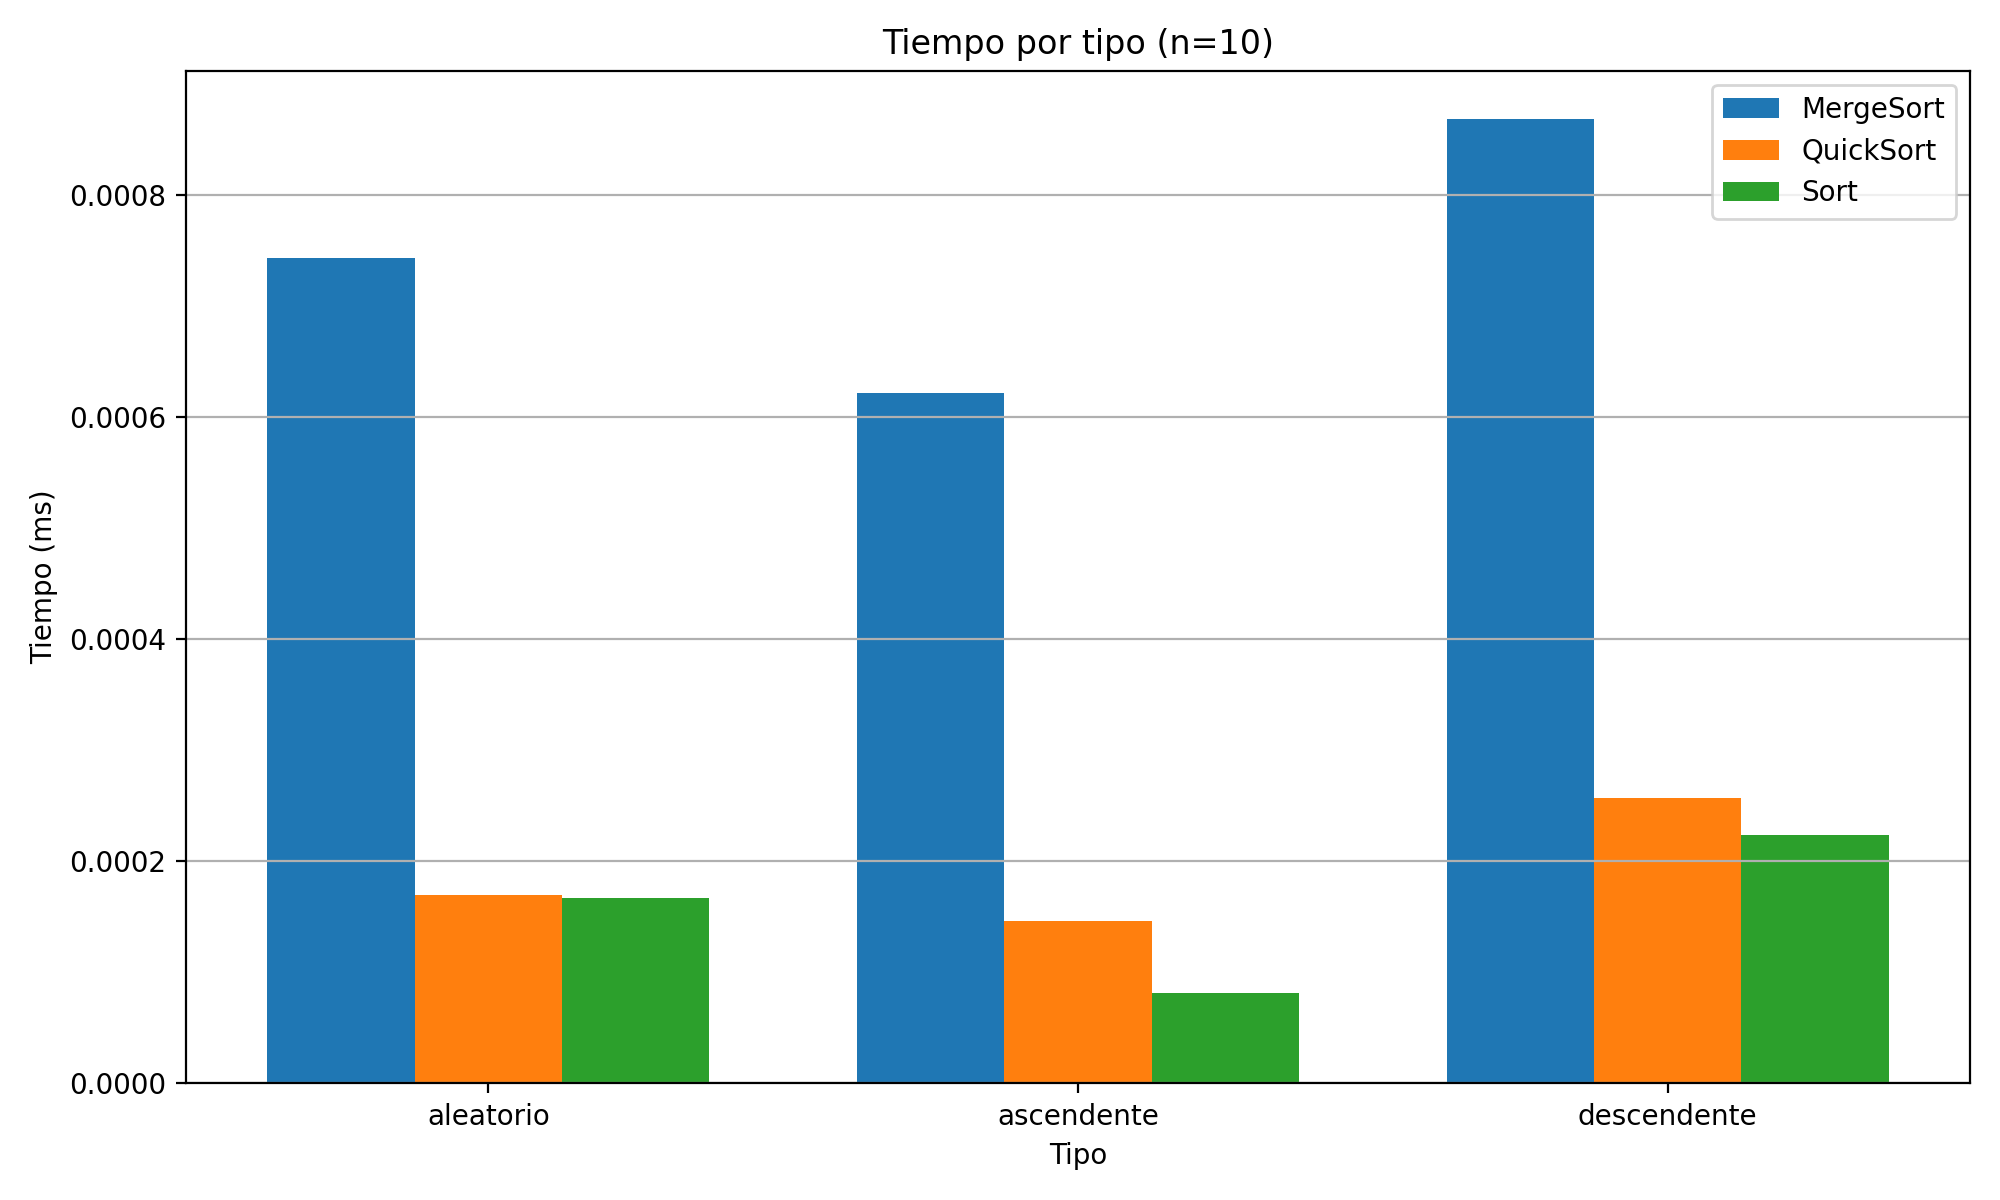
\includegraphics[width=\linewidth]{../code/sorting/data/plots/time_n10.png}
                \caption{Tiempos}
                \label{fig:img2}
            \end{subfigure}

        \end{minipage}
    }
    \caption{Resultados para n=$10^1$}
    \label{fig:comparacion n=$10^1$ sort}
\end{figure}
Para \(n = 10^1\), MergeSort utiliza cerca de \(4n\) bytes de memoria auxiliar, mientras que QuickSort y \texttt{Sort} no presentan uso significativo de heap. 
En tiempo de ejecución, MergeSort resulta ser el más lento en los tres casos, debido al costo de copiar y mezclar subarreglos. 
En cambio, QuickSort y \texttt{Sort} muestran tiempos menores y similares entre sí, con mejor desempeño en el caso ascendente y 
un leve aumento en el descendente, lo que puede explicarse por la forma en que la elección del pivote afecta el balance de las particiones.

\begin{figure}[H]
    \centering
    \resizebox{\textwidth}{!}{
        \begin{minipage}{\textwidth}
            \centering

            \begin{subfigure}{0.48\textwidth}
                \centering
                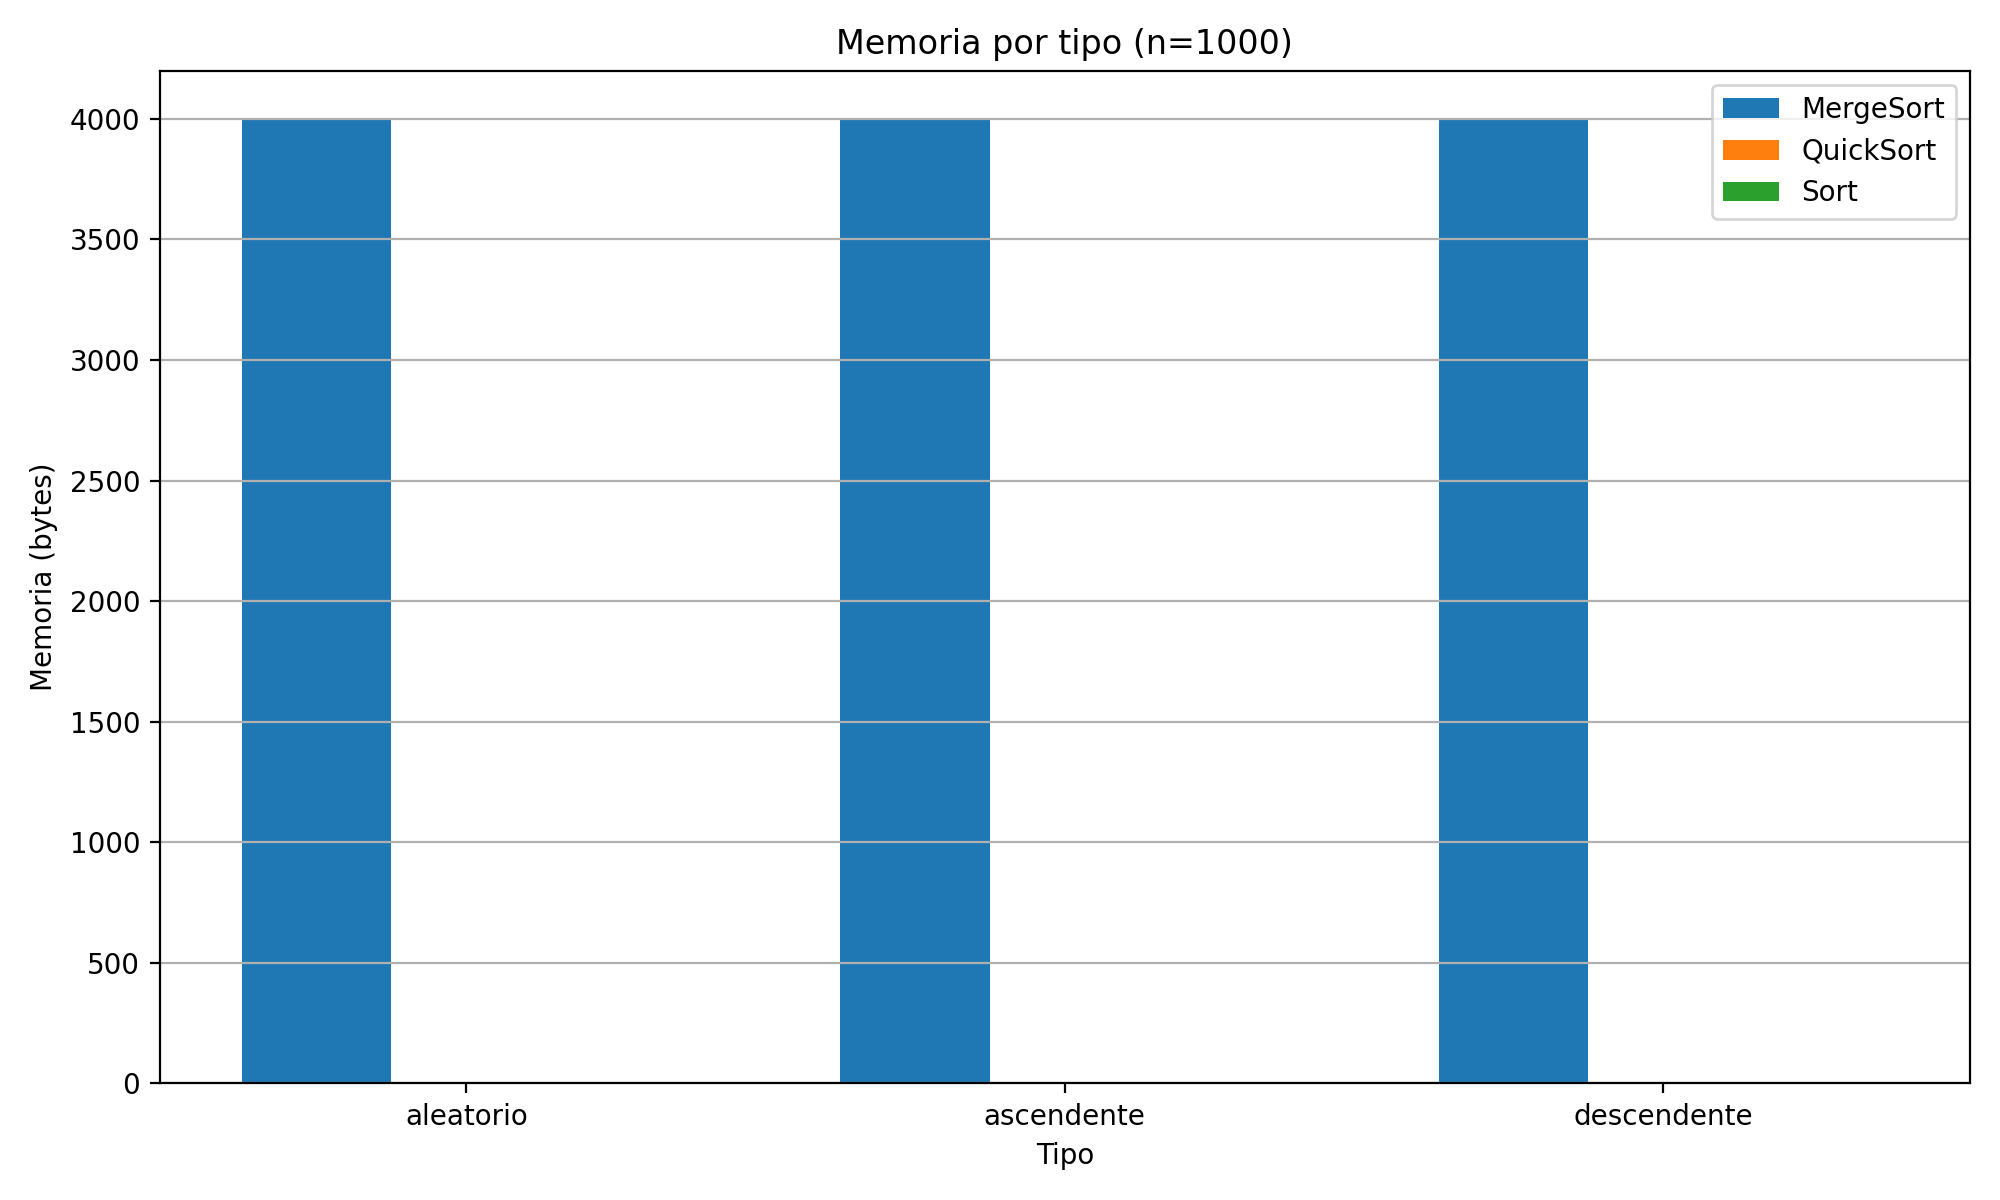
\includegraphics[width=\linewidth]{../code/sorting/data/plots/memory_n1000.png}
                \caption{Memoria}
                \label{fig:img3}
            \end{subfigure}
            \hfill
            \begin{subfigure}{0.48\textwidth}
                \centering
                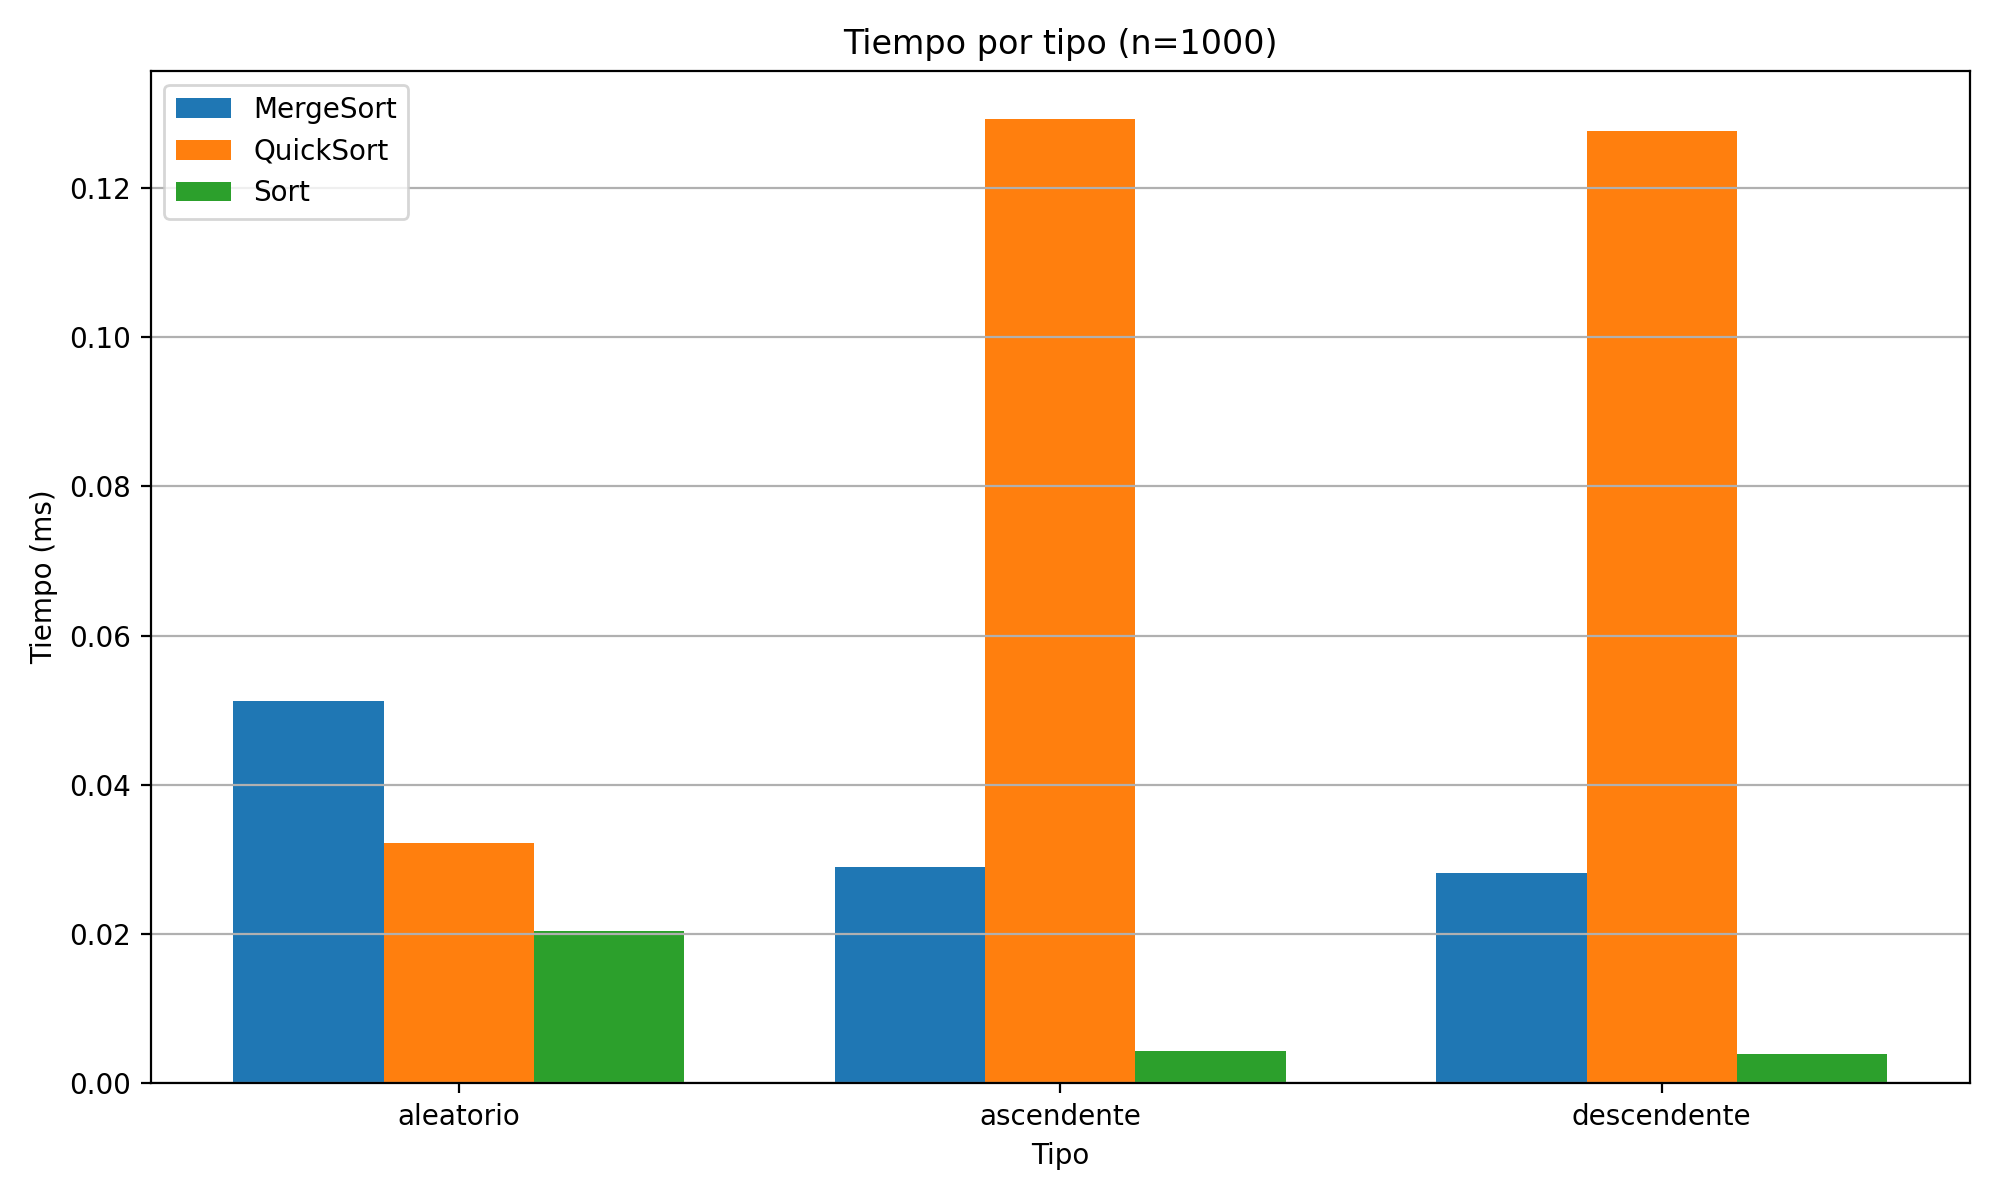
\includegraphics[width=\linewidth]{../code/sorting/data/plots/time_n1000.png}
                \caption{Tiempos}
                \label{fig:img4}
            \end{subfigure}

        \end{minipage}
    }
    \caption{Resultados para n=$10^3$}
    \label{fig:comparacion n=$10^3$ sort}
\end{figure}

Para \(n = 10^3\), MergeSort utiliza aproximadamente \(4n\) bytes de memoria auxiliar, mientras que QuickSort y 
\texttt{Sort} no presentan uso significativo de heap. En tiempo de ejecución, MergeSort mantiene un comportamiento estable en todos los casos.
QuickSort, en cambio, presenta un buen desempeño en el caso promedio, pero se degrada fuertemente en entradas ascendentes y descendentes 
debido a la mala elección de pivote. Finalmente, \texttt{Sort} obtiene los mejores tiempos en todos los casos, gracias a su 
implementación híbrida que evita el peor caso.

\begin{figure}[H]
    \centering
    \resizebox{\textwidth}{!}{
        \begin{minipage}{\textwidth}
            \centering

            \begin{subfigure}{0.48\textwidth}
                \centering
                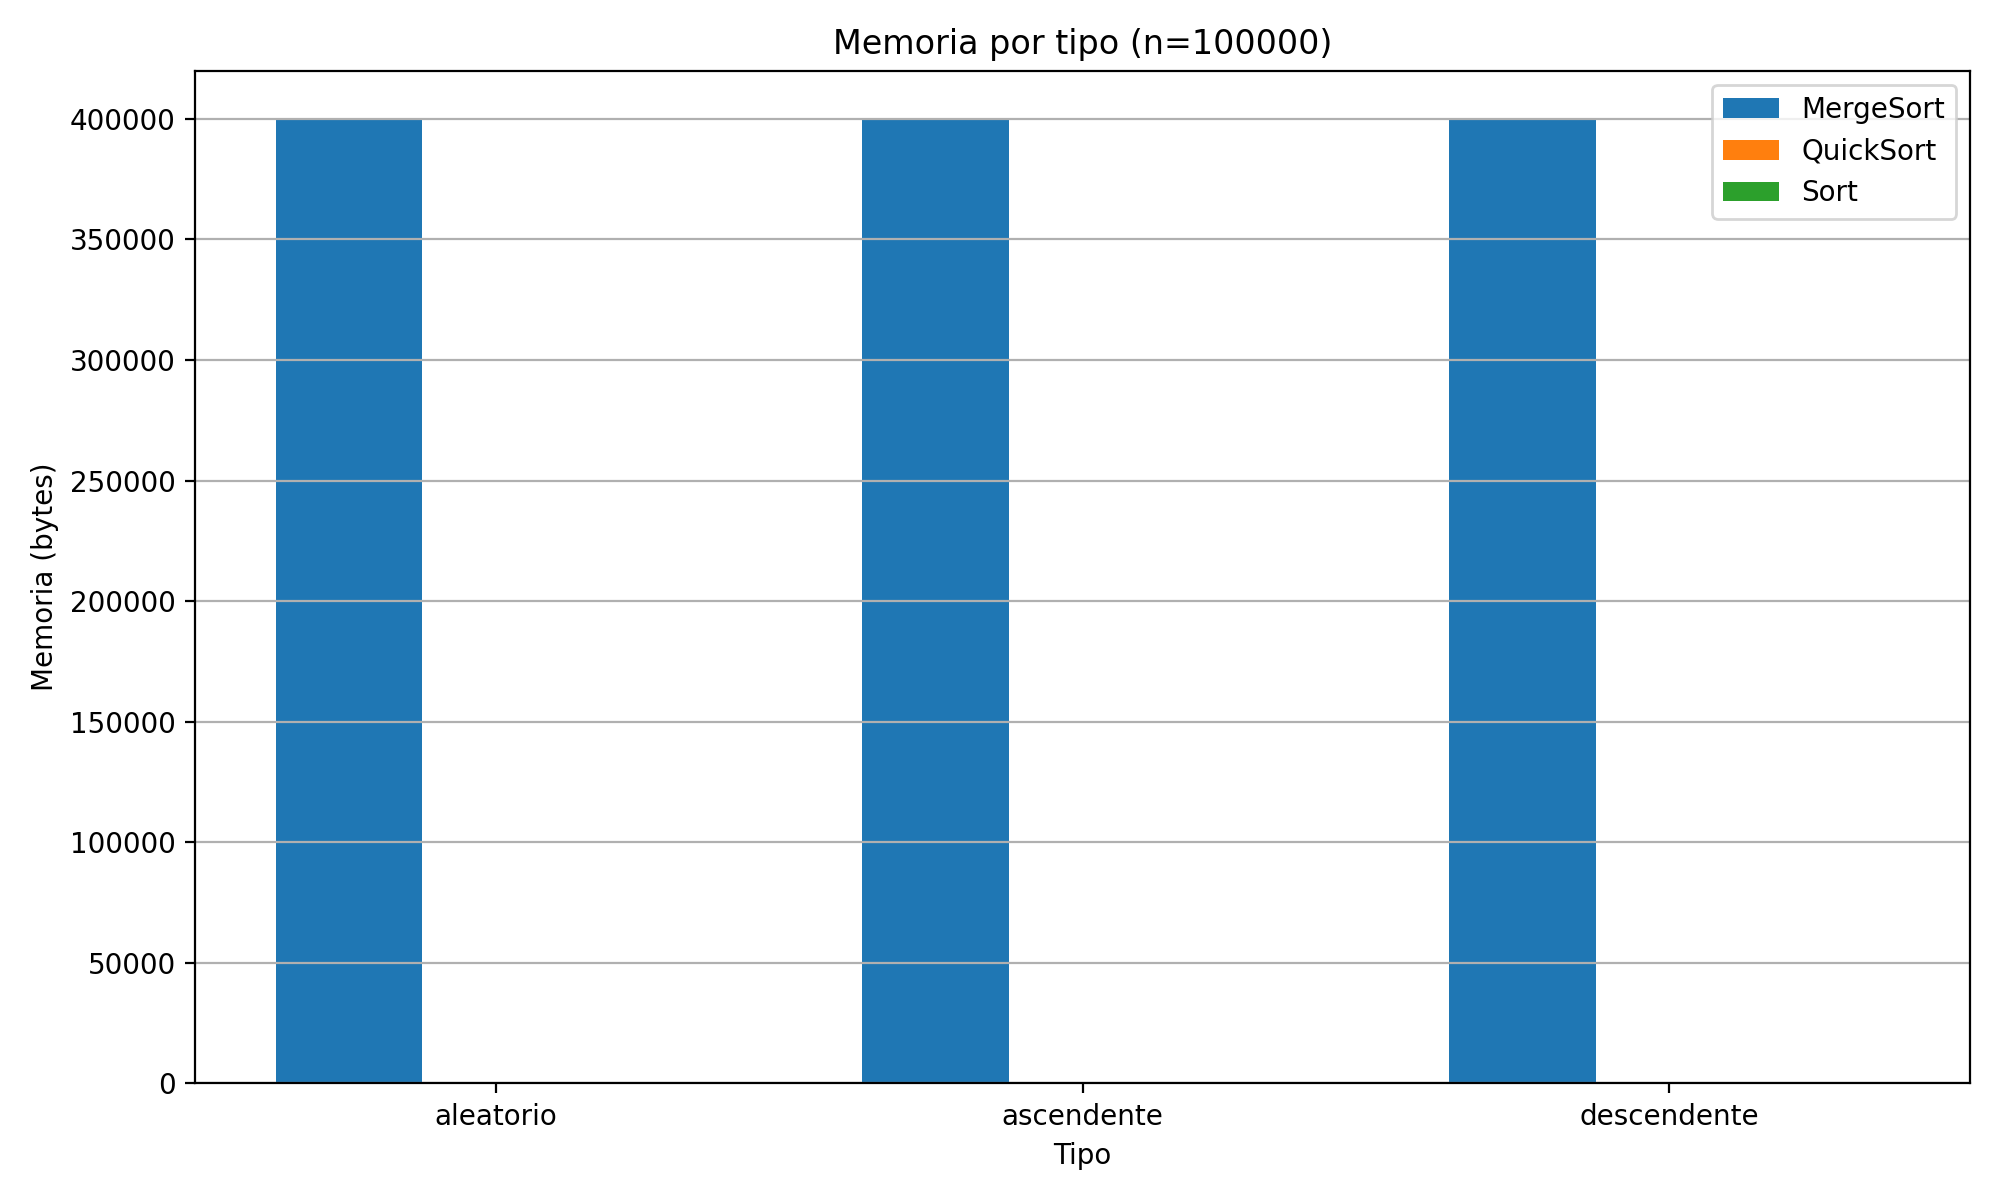
\includegraphics[width=\linewidth]{../code/sorting/data/plots/memory_n100000.png}
                \caption{Memoria}
                \label{fig:img5}
            \end{subfigure}
            \hfill
            \begin{subfigure}{0.48\textwidth}
                \centering
                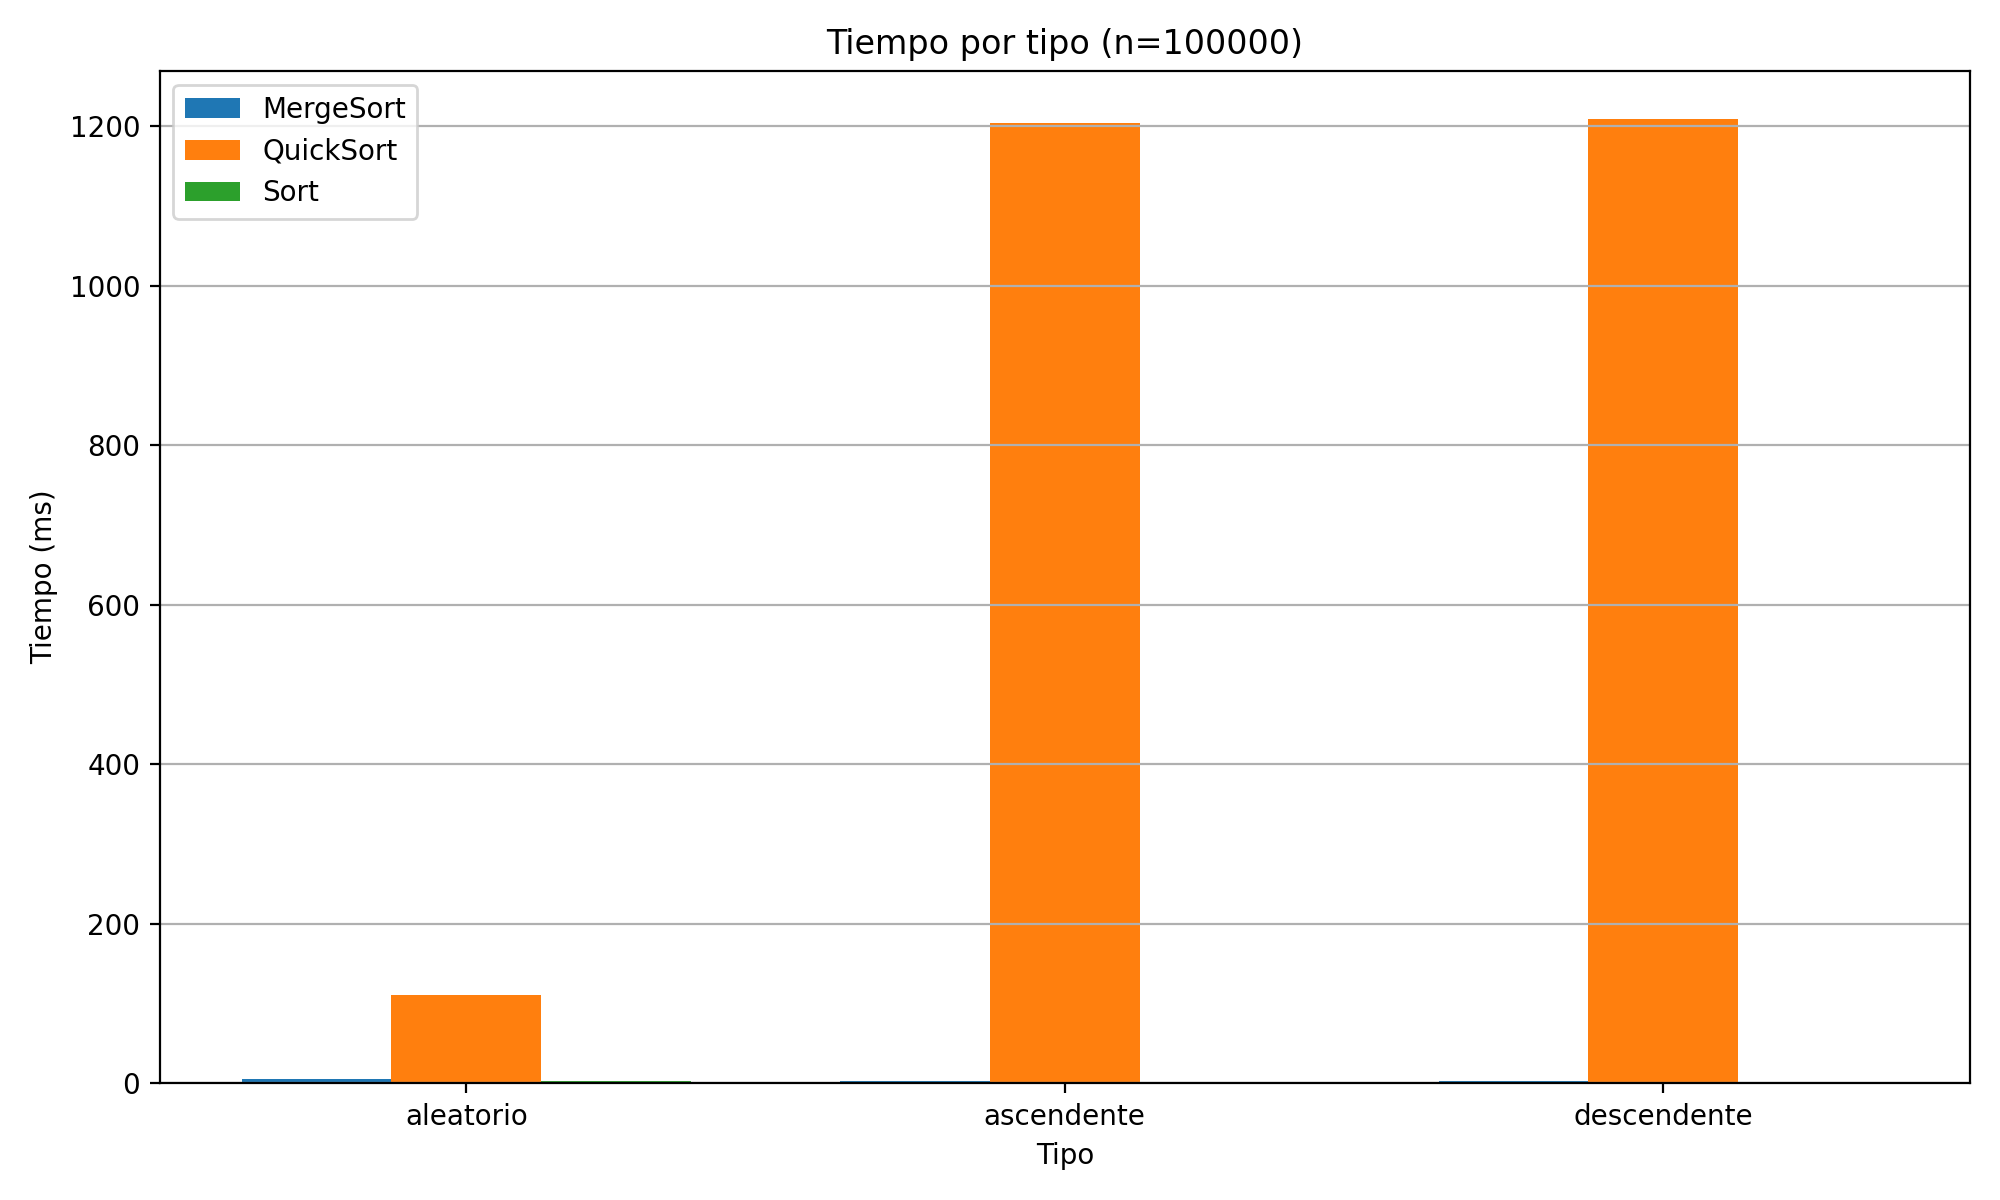
\includegraphics[width=\linewidth]{../code/sorting/data/plots/time_n100000.png}
                \caption{Tiempos}
                \label{fig:img6}
            \end{subfigure}

        \end{minipage}
    }
    \caption{Resultados para n=$10^5$}
    \label{fig:comparacion n=$10^5$ sort} 
\end{figure}
Para \(n = 10^5\), el comportamiento de la memoria se mantiene igual que en los casos anteriores. 
Sin embargo, destaca el bajo rendimiento de QuickSort en los casos ascendente y descendente, cuyos tiempos crecen de tal forma que 
dejan fuera de escala los de MergeSort y \texttt{sort} en la gráfica.
\\ 
En un análisis general, se observa que QuickSort presenta un mal rendimiento cuando el arreglo está ordenado de forma ascendente o 
descendente, ya que en estos casos su complejidad se degrada a \(O(n^2)\), lo que se acentúa al aumentar \(n\). 
Por otro lado, \texttt{sort} mantiene un buen desempeño en todos los casos gracias a su implementación híbrida, 
que evita el peor caso de QuickSort. Finalmente, MergeSort presenta tiempos estables independientes del tipo de entrada, aunque su 
principal desventaja es el uso de memoria adicional proporcional al tamaño del arreglo.
\\ 
A continuación, se presenta el análisis de los algoritmos de multiplicación de matrices.
\begin{figure}[H]
    \centering
    \resizebox{\textwidth}{!}{
        \begin{minipage}{\textwidth}
            \centering

            \begin{subfigure}{0.48\textwidth}
                \centering
                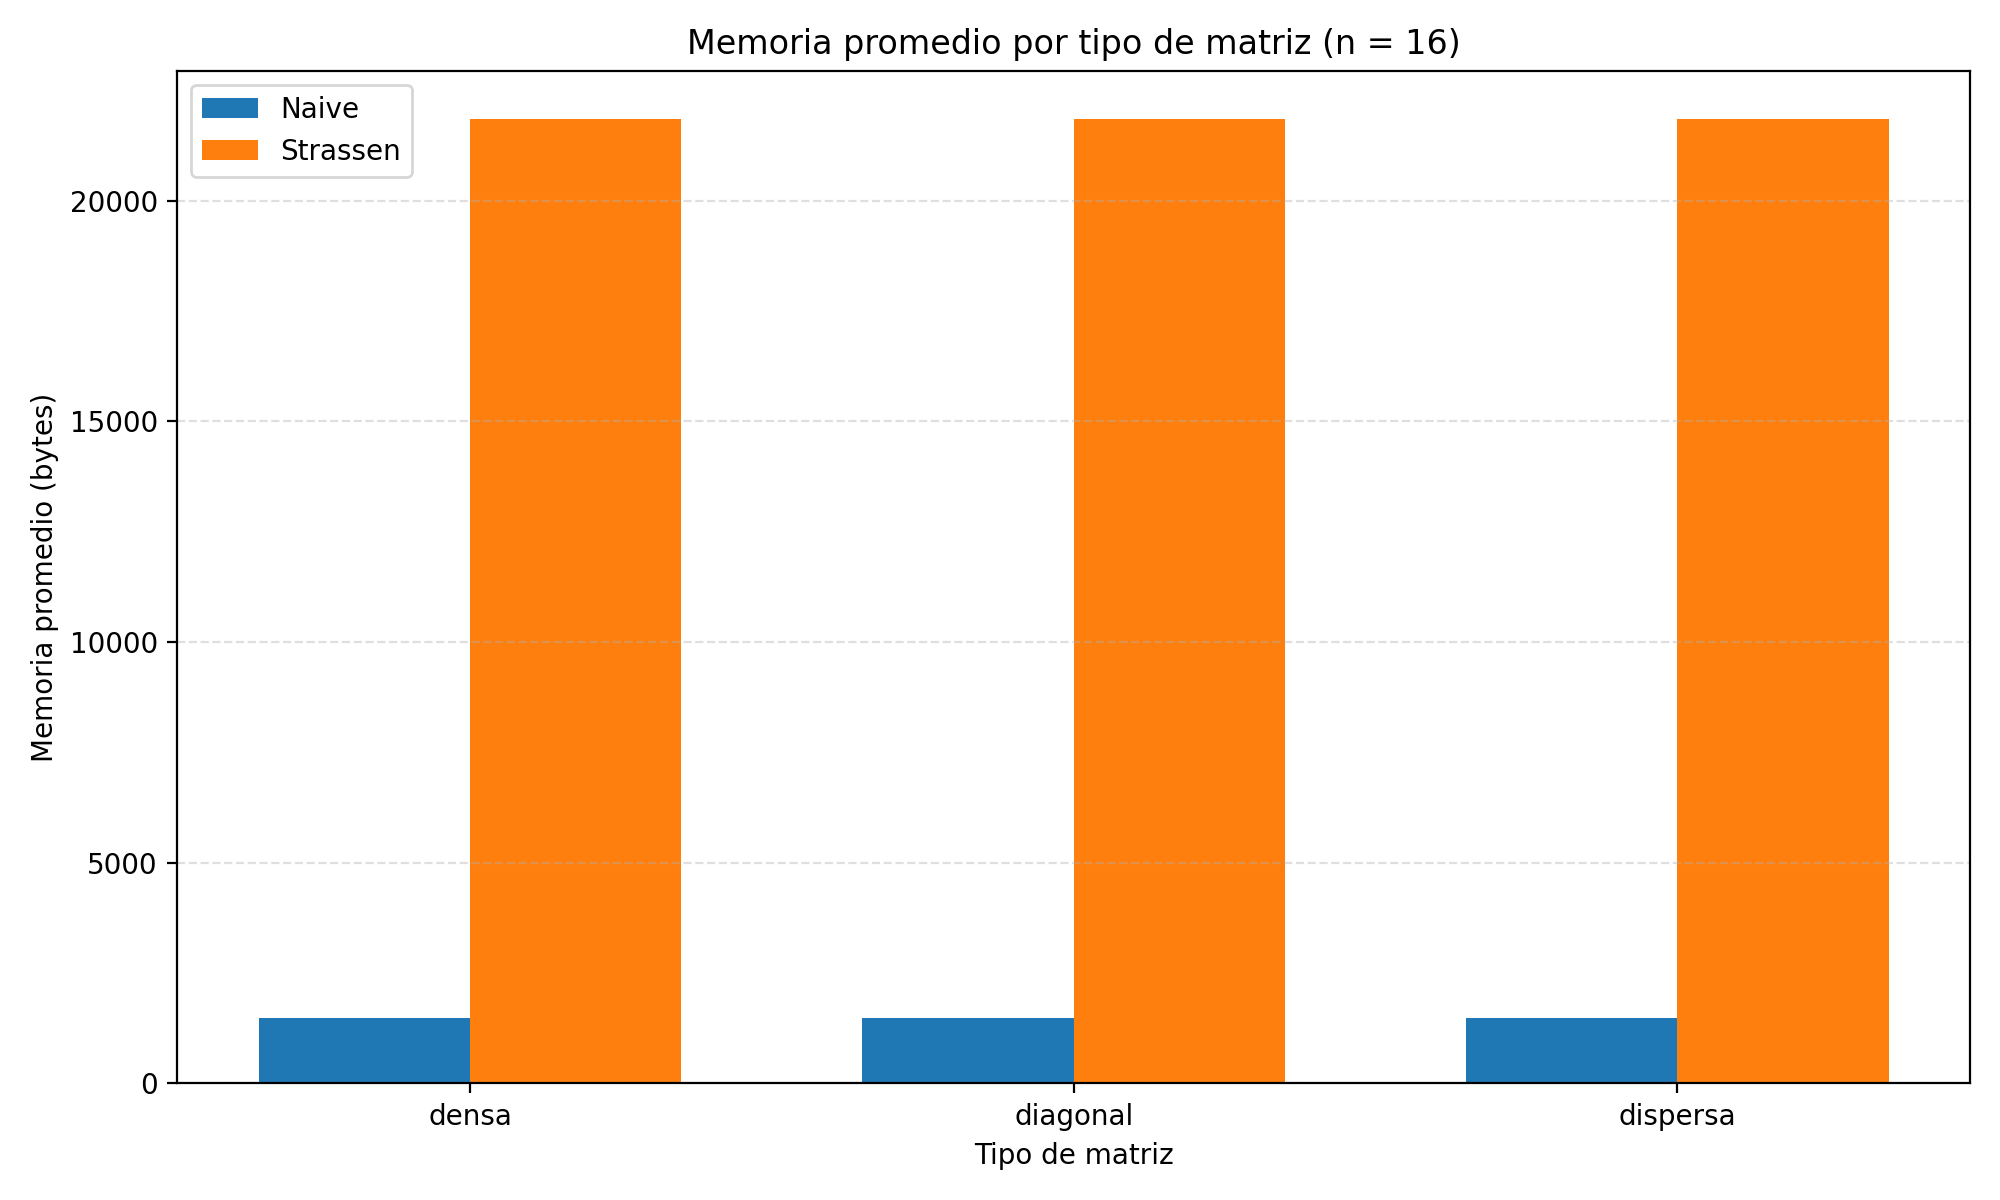
\includegraphics[width=\linewidth]{../code/matrix_multiplication/data/plots/matrix_barras_memoria_n16.png}
                \caption{Memoria}
                \label{fig:img7}
            \end{subfigure}
            \hfill
            \begin{subfigure}{0.48\textwidth}
                \centering
                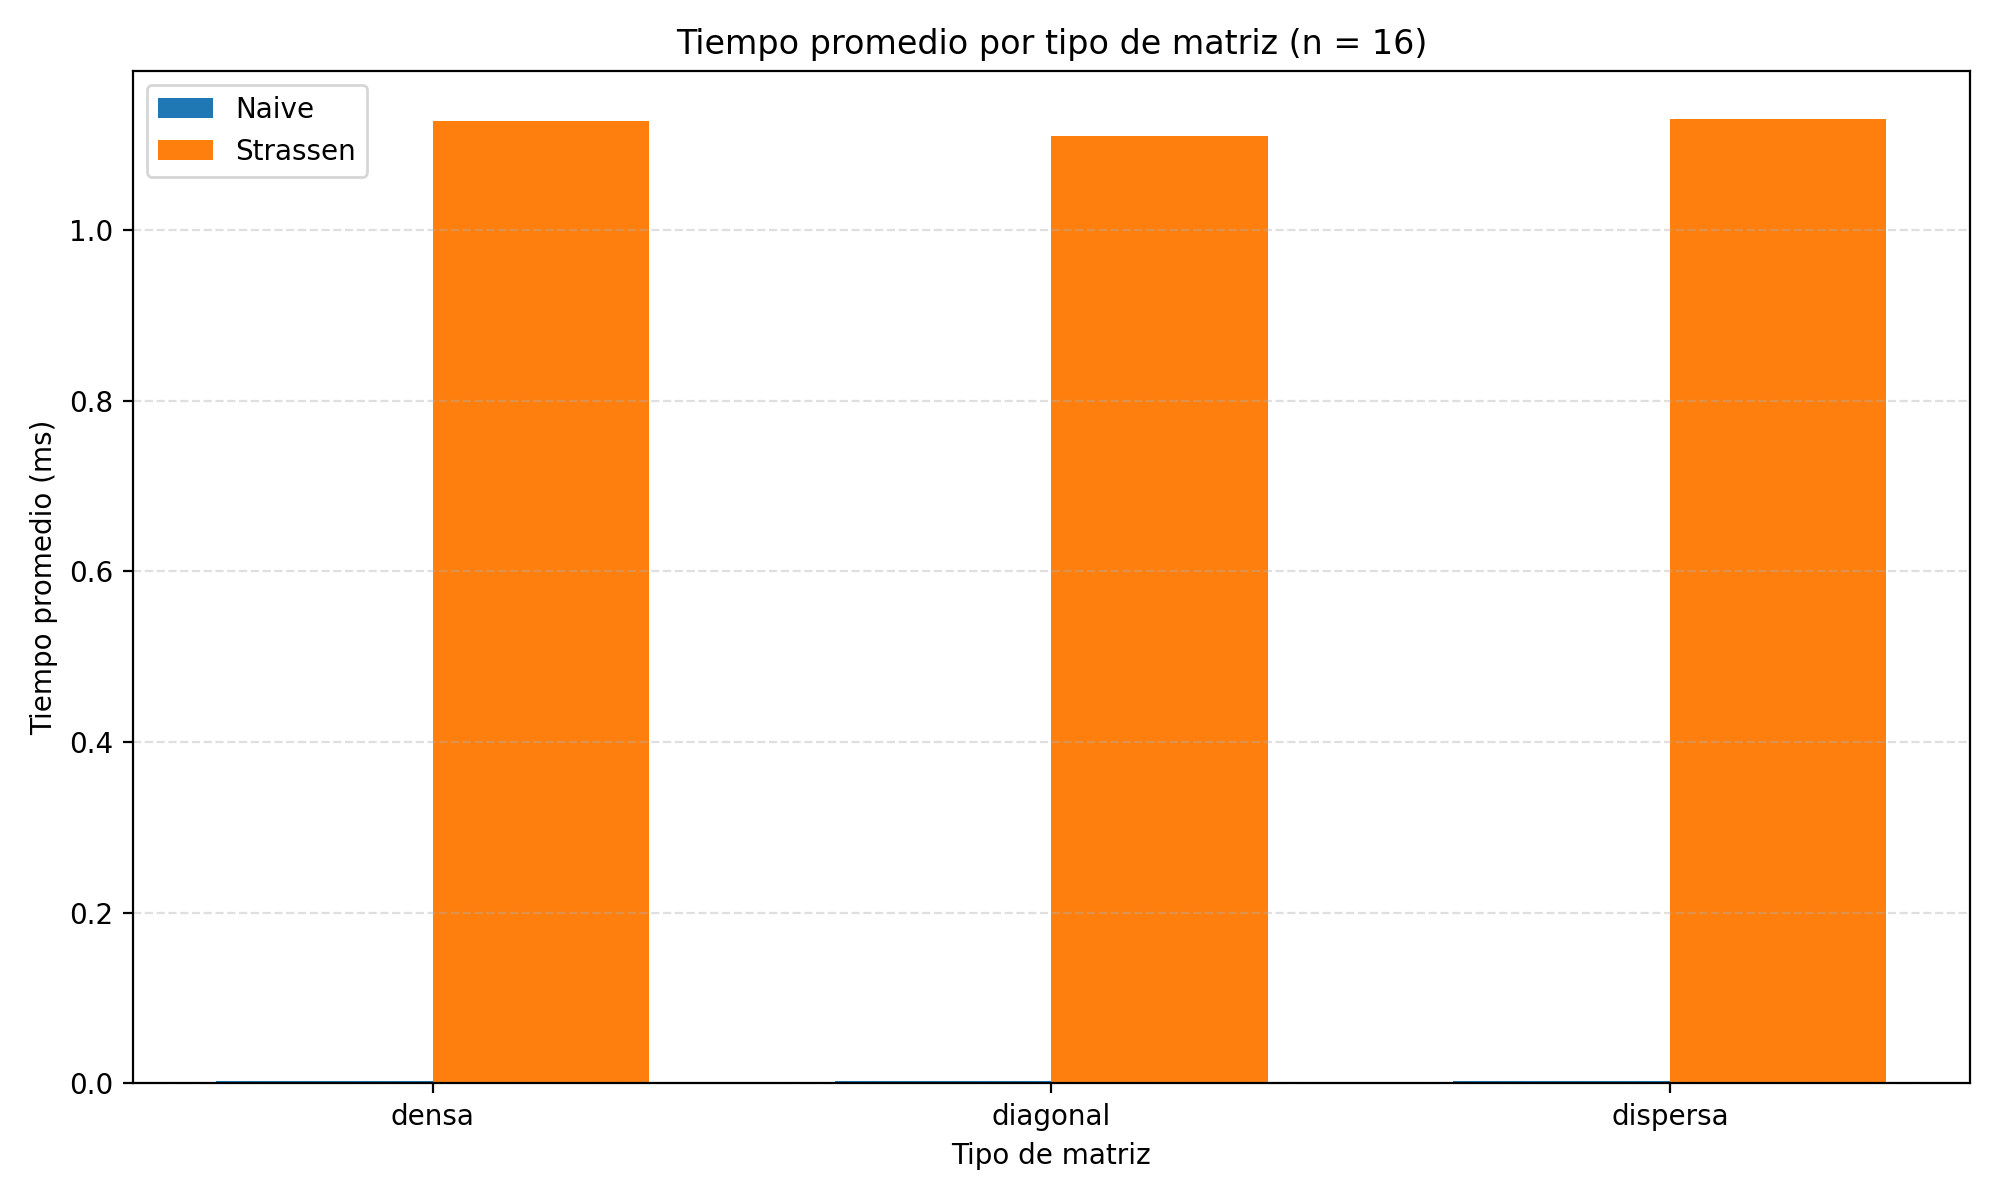
\includegraphics[width=\linewidth]{../code/matrix_multiplication/data/plots/matrix_barras_tiempo_n16.png}
                \caption{Tiempos}
                \label{fig:img8}
            \end{subfigure}

        \end{minipage}
    }
    \caption{Resultados para matrices 16x16}
    \label{fig:comparacion 16x16 matrix}
\end{figure}
Para \(n = 16\), se observa que Strassen utiliza considerablemente más memoria que el algoritmo naive en todos los tipos de matrices. 
En cuanto al tiempo de ejecución, el algoritmo naive es claramente más rápido, mientras que Strassen presenta un mayor costo debido al 
overhead de su implementación recursiva.

\begin{figure}[H]
    \centering
    \resizebox{\textwidth}{!}{
        \begin{minipage}{\textwidth}
            \centering

            \begin{subfigure}{0.48\textwidth}
                \centering
                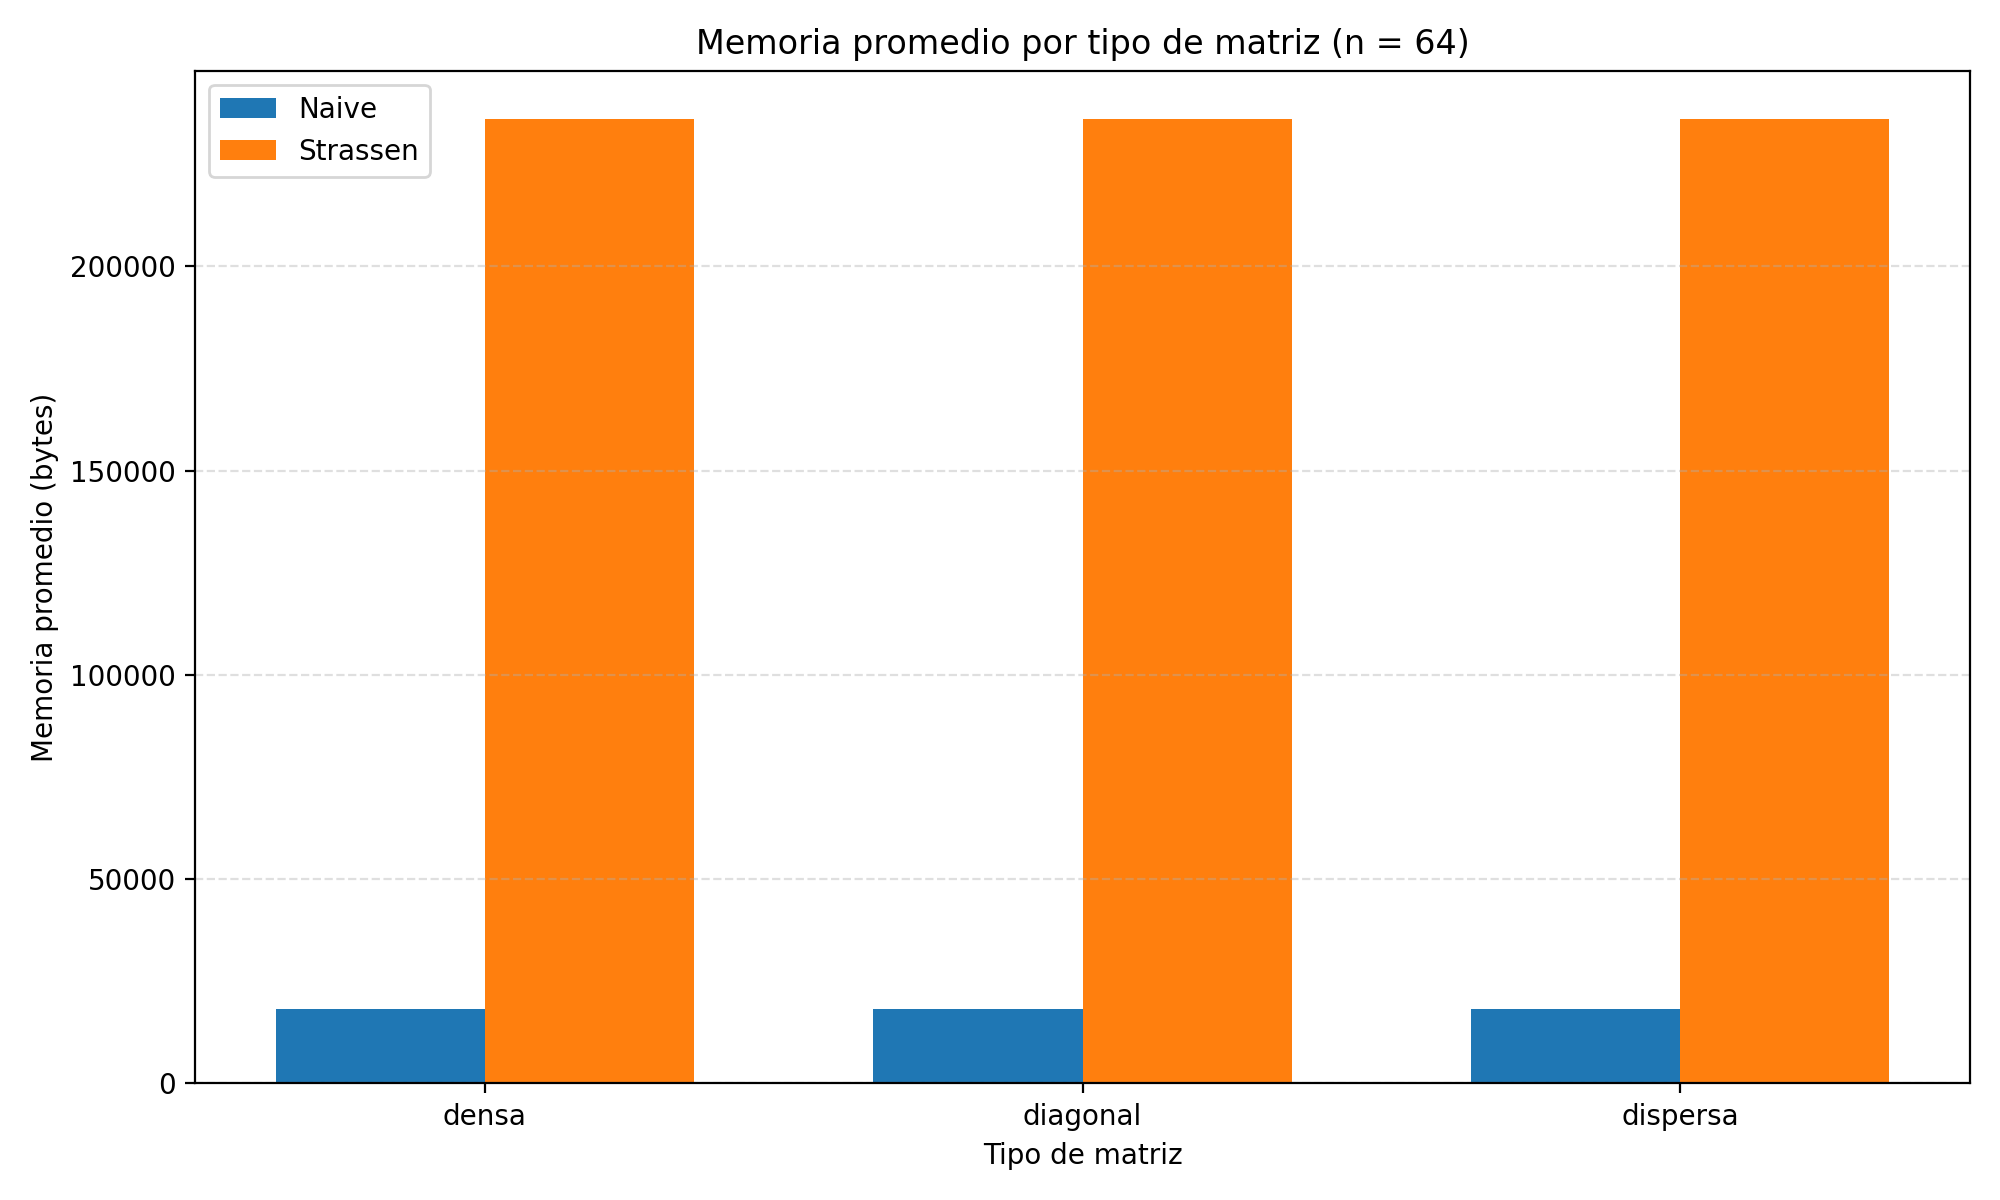
\includegraphics[width=\linewidth]{../code/matrix_multiplication/data/plots/matrix_barras_memoria_n64.png}
                \caption{Memoria}
                \label{fig:img9}
            \end{subfigure}
            \hfill
            \begin{subfigure}{0.48\textwidth}
                \centering
                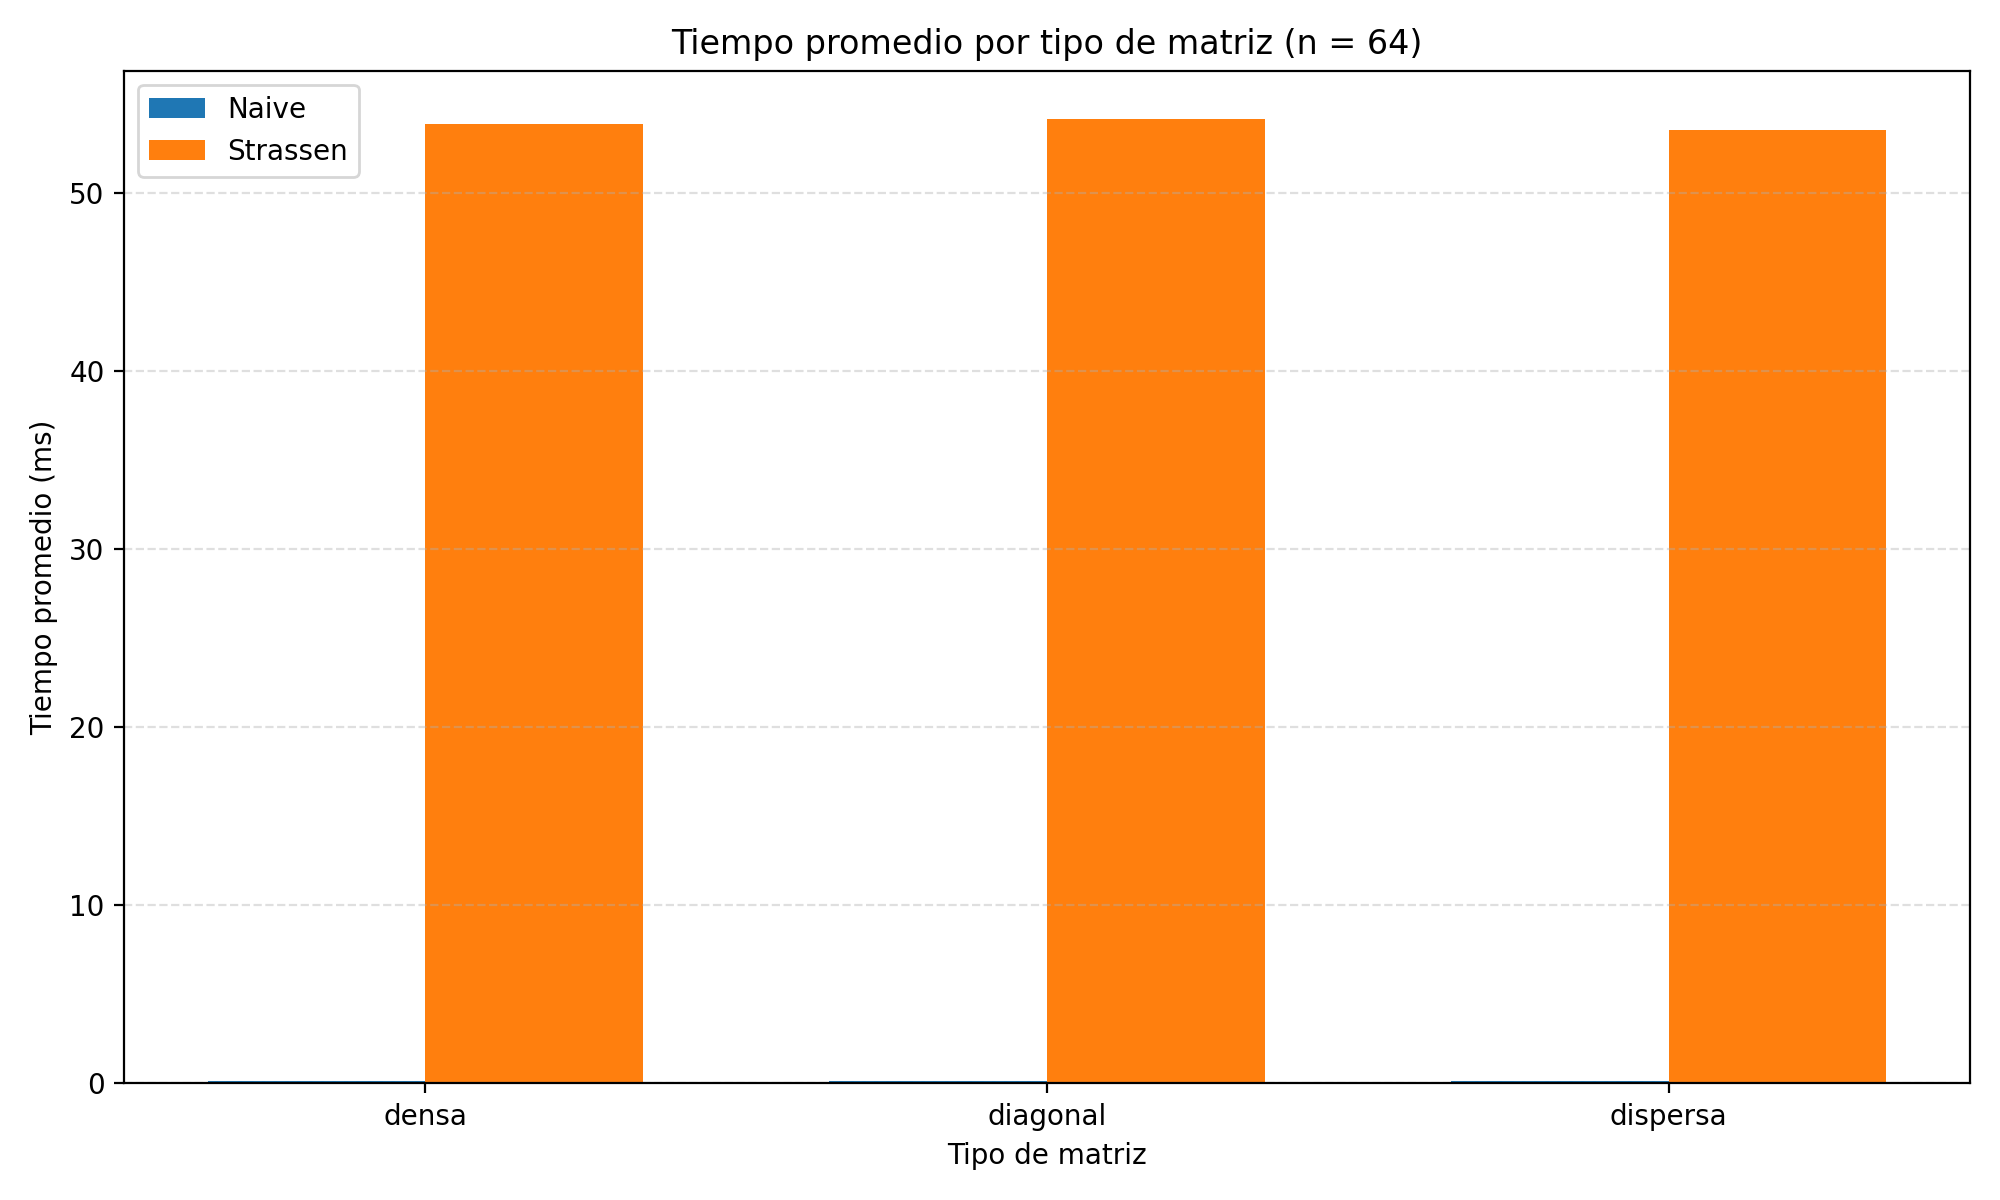
\includegraphics[width=\linewidth]{../code/matrix_multiplication/data/plots/matrix_barras_tiempo_n64.png}
                \caption{Tiempos}
                \label{fig:img10}
            \end{subfigure}

        \end{minipage}
    }
    \caption{Resultados para matrices 64x64}
    \label{fig:comparacion 64x64 matrix}
\end{figure}
Para \(n = 64\), se mantiene la misma tendencia observada anteriormente. Los gráficos presentan proporciones similares, 
aunque cambia la escala, ya que tanto el uso de memoria como los tiempos de ejecución aumentan para ambos algoritmos.


\begin{figure}[H]
    \centering
    \resizebox{\textwidth}{!}{
        \begin{minipage}{\textwidth}
            \centering

            \begin{subfigure}{0.48\textwidth}
                \centering
                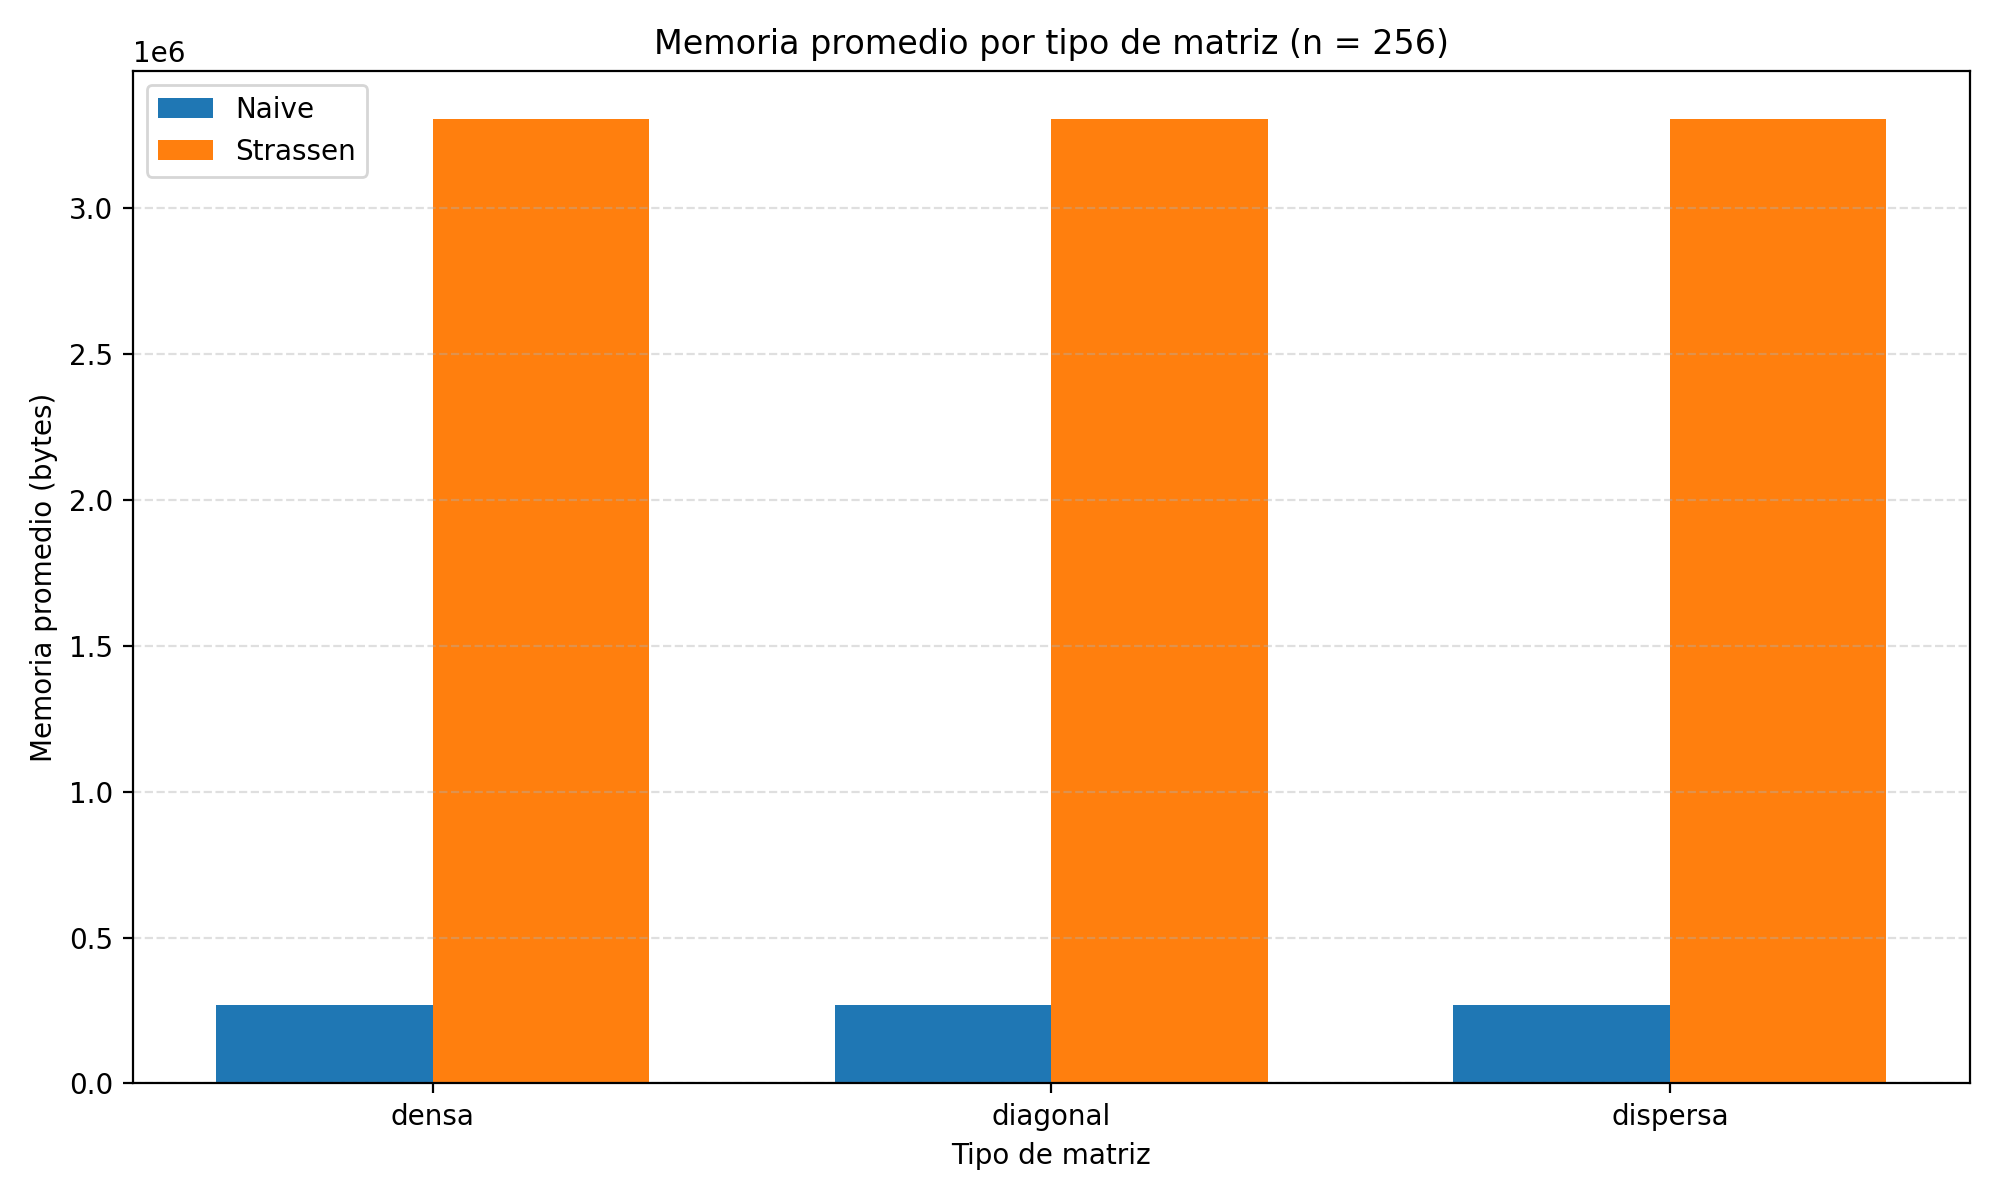
\includegraphics[width=\linewidth]{../code/matrix_multiplication/data/plots/matrix_barras_memoria_n256.png}
                \caption{Memoria}
                \label{fig:img11}
            \end{subfigure}
            \hfill
            \begin{subfigure}{0.48\textwidth}
                \centering
                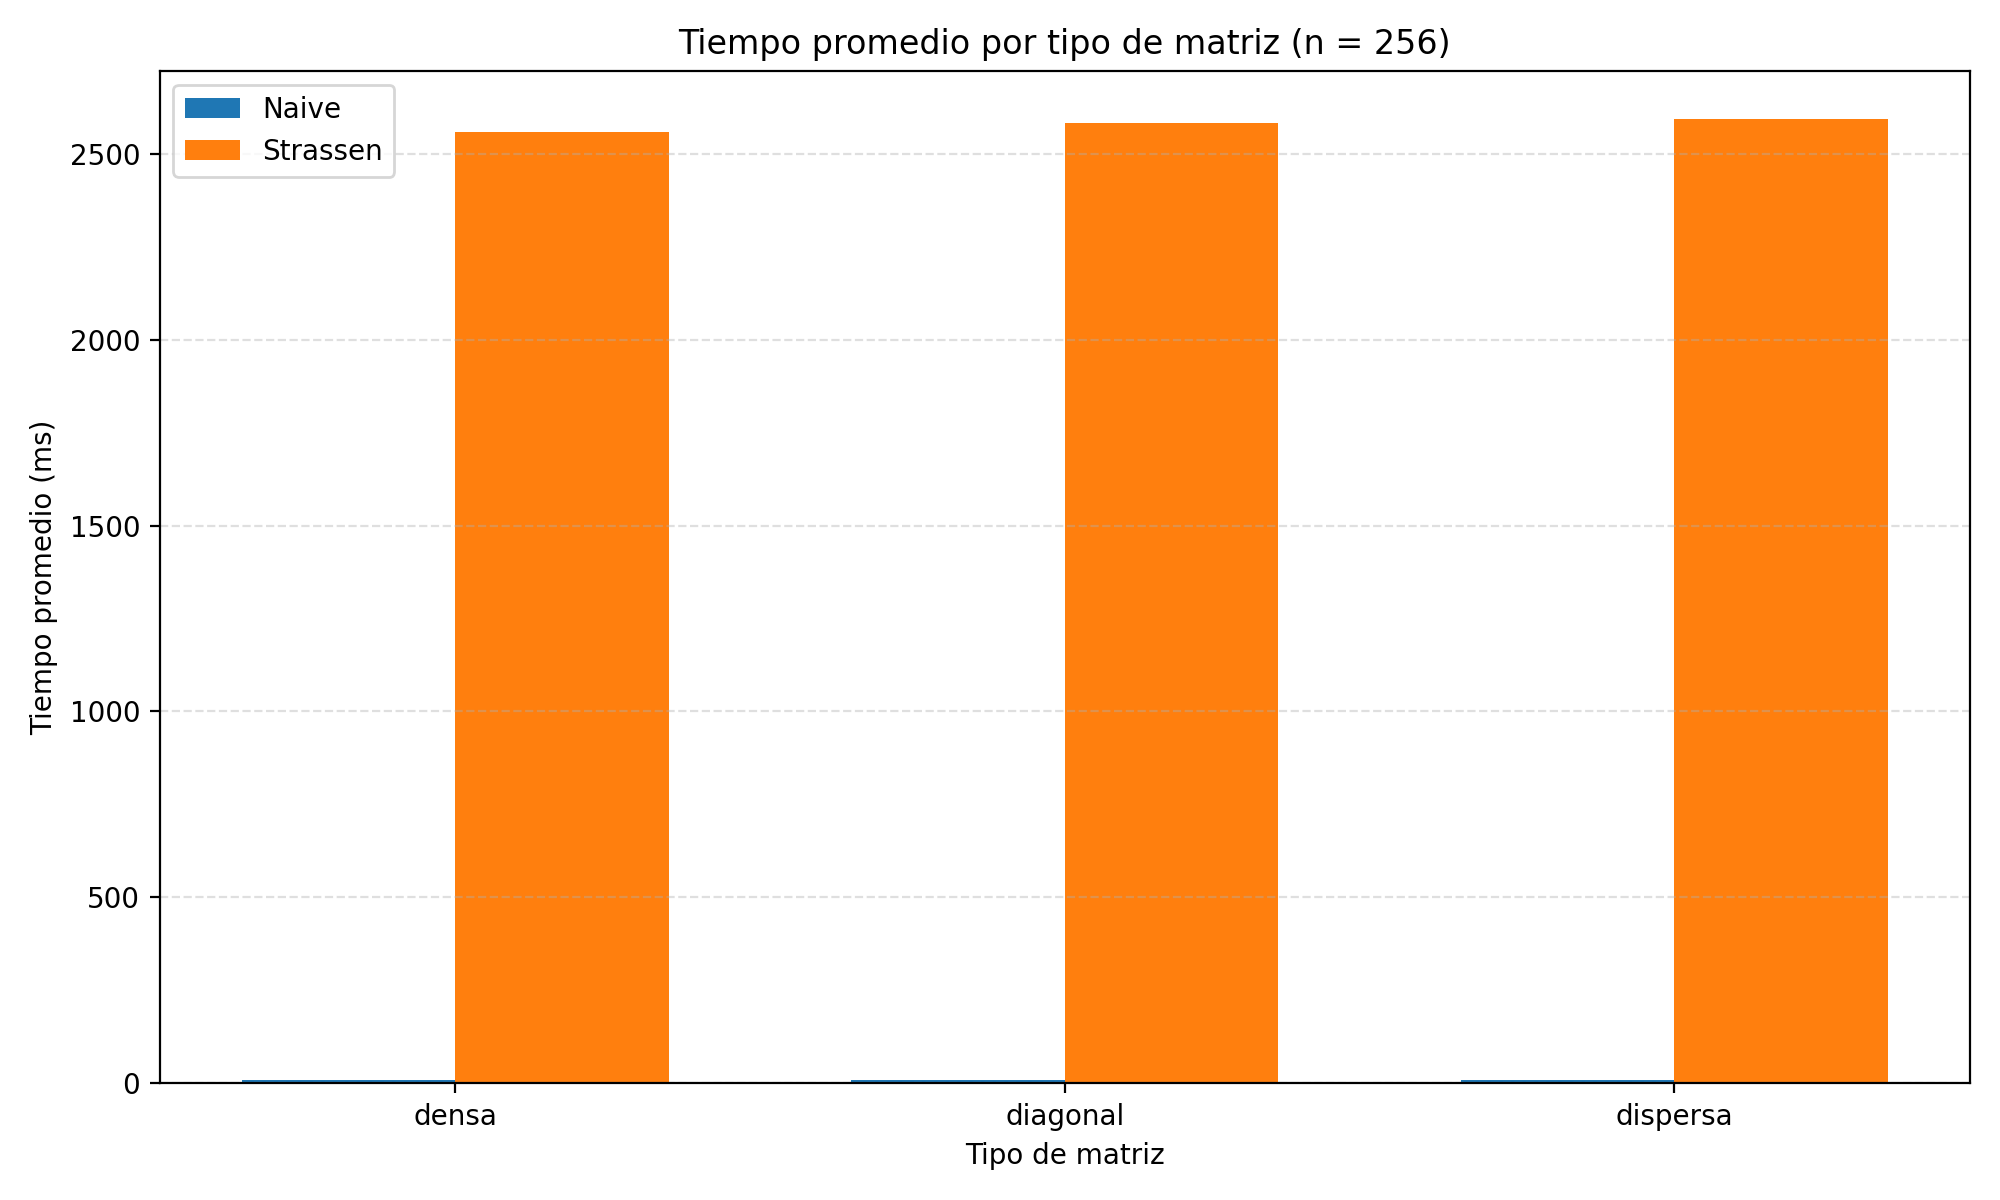
\includegraphics[width=\linewidth]{../code/matrix_multiplication/data/plots/matrix_barras_tiempo_n256.png}
                \caption{Tiempos}
                \label{fig:img12}
            \end{subfigure}

        \end{minipage}
    }
    \caption{Resultados para matrices 256x256}
    \label{fig:comparacion 256x256 matrix}
\end{figure}
Para \(n = 256\), el uso de memoria aumenta considerablemente, lo que provoca un cambio en la escala del gráfico para poder 
representar ambas implementaciones. En cuanto al tiempo de ejecución, el algoritmo naive incrementa ligeramente su tiempo respecto a 
casos anteriores; sin embargo, debido a la gran diferencia con Strassen, este aumento no se aprecia claramente en la gráfica.

\vspace{0.5cm}
Para interpretar estos resultados, es importante destacar que el algoritmo de Strassen tuvo un mal desempeño debido a la en esta igual
implementación. A pesar de que teóricamente presenta una mejor complejidad que el método naive, en la práctica su rendimiento depende 
fuertemente de factores como los costos constantes y el manejo de memoria.
En particular, la implementación utilizada introduce un alto overhead debido a que las matrices se pasan por valor en las llamadas 
recursivas, generando copias completas en cada nivel. Además, el algoritmo divide las matrices en múltiples submatrices y crea 
estructuras auxiliares para las operaciones intermedias, lo que incrementa significativamente el uso de memoria dinámica.
Este comportamiento es consistente con lo indica la referencia utilizada para la implementación del algoritmo,
donde se menciona que el método de Strassen suele presentar altos costos constantes y requerimientos adicionales de memoria, lo que puede hacerlo menos eficiente que el algoritmo naive en tamaños 
moderados. Por esta razón, en los experimentos realizados, la sobrecarga de implementación domina sobre la mejora teórica, resultando en 
un peor desempeño tanto en tiempo como en uso de memoria.

\newpage
